\documentclass[a4paper]{article}

\usepackage[utf8]{inputenc}
\usepackage[portuges]{babel}
\usepackage{indentfirst}
\usepackage{graphicx}
\usepackage{float}
\usepackage{caption}
\usepackage{subcaption}
\usepackage[T1]{fontenc}
\usepackage{listings}
\usepackage{amsmath}
\usepackage{mathtools}
\renewcommand{\familydefault}{\sfdefault}


\title{Projeto de Computação Gráfica - Fase 2}
\author{Diogo Braga A82547 \and João Silva A82005 \and Ricardo Caçador A81064
\and Ricardo Veloso A81919}
\date{\today}

\begin{document}

\maketitle

\begin{abstract}
Neste relatório é apresentada a segunda fase dum projeto no qual a intenção é desenvolver um mecanismo baseado em gráficos 3D e fornecer exemplos de uso que mostrem o seu potencial. Este projeto é desenvolvido no âmbito da unidade curricular de Computação Gráfica.
\end{abstract}


\newpage

\tableofcontents


\newpage

\section{Introdução}
\label{sec:intro}

Esta segunda fase tem como objetivo a realização de algumas etapas, nomeadamente:
\begin{enumerate}
\item A criação dum parser \emph{XML} mais conciso;
\item A alteração/evolução da estrutura dos ficheiros \emph{XML};
\item A criação de estruturas capazes de armazenar as figuras necessárias;
\item A criação de funções que leiam as estruturas e as desenhem;
\item A criação dum modelo estático do sistema solar.
\end{enumerate}

De seguida iremos apresentar todos os algoritmos e decisões relativos à realização destas etapas, bem como as respetivas explicações de cada passo.
Serão ainda apresentadas figuras e esquemas que ilustrem os passos do processo desenvolvido.



\section{Estrutura da Pasta do Projeto}
\label{sec:estrutura}

Para um entendimento mais claro da estrutura do projeto, achamos por bem referenciar a estrutura da pasta do projeto.
O projeto entregue contêm para além do relatório, 4 pastas como é possível verificar na seguinte figura.

\begin{figure}[H]
\centering
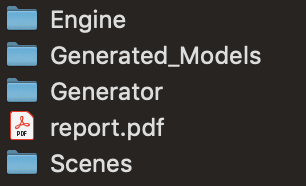
\includegraphics[scale=1.0]{estrutura.png}
\caption{Estrutura da pasta.}
\label{img:estrutura}
\end{figure}

Na pasta \textbf{Engine} residem os ficheiros relativos ao programa \emph{engine}, bem como as bibliotecas (.h) criadas para o efeito. Contém ainda um ficheiro de configuração \emph{cmake} e os ficheiros relativos à biblioteca \emph{tinyxml2}.

Na pasta \textbf{Generator} residem os ficheiros relativos ao programa \emph{generator}. Contém também um ficheiro de configuração \emph{cmake}.

Na pasta \textbf{Generated\_Models} residem os ficheiros que contêm os pontos gerados para cada figura, criados pelo programa \emph{generator}.

Na pasta \textbf{Scenes} residem os ficheiros \emph{XML} que contêm as estruturas do sistemas solares desenvolvidos para esta fase do projeto. Construímos dois ficheiros deste tipo, um que contém os raios relativos de cada planeta e do sol baseados na realidade (grande disparidade entre as figuras criadas), e o outro que é mais elucidativo e percetível.


\newpage

\section{Parser XML}
\label{sec:parser}

\subsection{Ficheiro}
\label{sec:ficheiro}

Devido aos requerimentos desta fase, foi necessário criar um novo ficheiro XML com o intuito de representar o sistema solar, que inclui: o sol, os planetas, e os satélites naturais destes mesmos.

Esta nova cena é encabeçada pelo grupo que faz referencia ao sol, e possui vários sub-grupos. Estes sub-grupos são referentes aos planetas, e possuem também sub-grupos. Estes sub-grupos dos planetas são referentes aos satélites naturais que cada um possui.

Todos os sub-grupos herdam as transformações geométricas presentes no grupo ao qual pertencem. Nesta fase, estas transformações são: translações, rotações e escalas.

Na figura \ref{img:ficheiro_parser} é possível visualizar um excerto do ficheiro XML por nós usado no qual constam o Sol, a Terra e a Lua.

\begin{figure}[H]
\centering
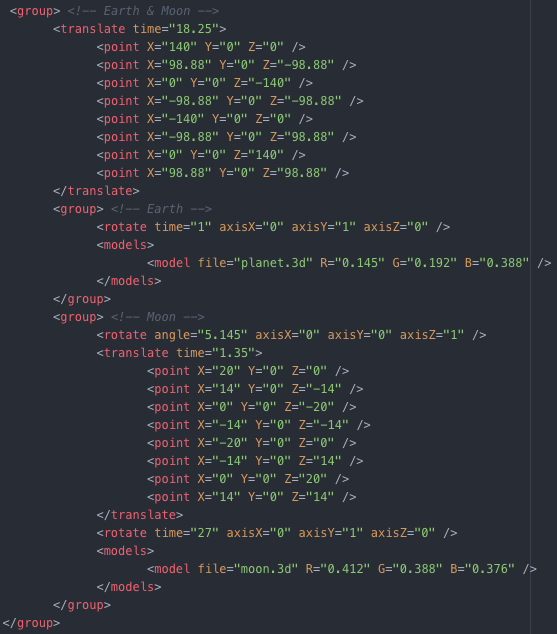
\includegraphics[scale=0.6]{ficheiro_parser.png}
\caption{Exemplo dum ficheiro usado no Parser.}
\label{img:ficheiro_parser}
\end{figure}

De referenciar que para facilitar a parte de coloração de cada corpo do sistema solar, acrescentamos ao \textbf{model} 3 novos valores que se referem à cor que determinado objeto terá. Estes campos são nomeadamente \textbf{R}, \textbf{G} e \textbf{B}.

\subsection{Funcionamento}
\label{sec:funcionamento}

O parser é inicializado na função \textbf{parser\_XML}. Esta função tem a principal funcionalidade de atualizar a variável global \textbf{Tree t}, sendo esta a estrutura que irá armazenar a informação retirada do ficheiro XML. O algoritmo deste processo é demonstrado a seguir:

    \vspace{0.5cm}

  Função parser\_XML:

    \vspace{0.1cm}

\ttfamily
\begin{enumerate}
 \item Abre ficheiro $\Rightarrow$ "scene.xml"
    \begin{enumerate}
      \item Caso resulte em erro, termina execução.
    \end{enumerate}
 \item Filtra primeiro elemento $\Rightarrow$ scene
    \begin{enumerate}
      \item Caso não seja obtido, termina execução.
    \end{enumerate}
 \item A partir do nodo atual, procura o primeiro filho, $\Rightarrow$ group
    \begin{enumerate}
      \item Caso não seja obtido, termina execução.
    \end{enumerate}
 \item O nodo (group) obtido no passo anterior é usado como parâmetro na função parseGroup.
\end{enumerate}

  \vspace{0.3cm}

 Função parseGroup:

  \vspace{0.3cm}

\begin{enumerate}
 \item Iterar sobre todos os filhos do nodo passado como parâmetro, até algum ser null:

   \begin{enumerate}
     \item Caso seja translate:
        \begin{enumerate}
          \item Obtém os valores e atribui-os à figura $\Rightarrow$ X,Y,Z
        \end{enumerate}
     \item Caso seja rotate:
        \begin{enumerate}
          \item Obtém os valores e atribui-os à figura $\Rightarrow$ angle,X,Y,Z
        \end{enumerate}
     \item Caso seja scale:
        \begin{enumerate}
          \item Obtém os valores e atribui-os à figura $\Rightarrow$ X,Y,Z
        \end{enumerate}
     \item Caso seja models:
        \begin{enumerate}
          \item Iterar sobre os nodos filhos existentes:
              \begin{enumerate}
                \item Obtém o nome do ficheiro da figura e invoca com esse parâmetro a função $\Rightarrow$ loadFigure
                \item Obtém os valores das cores e atribui-os à figura $\Rightarrow$ R,G,B
              \end{enumerate}
        \end{enumerate}

    \vspace{0.3cm}

  Função loadFigure:

    \vspace{0.3cm}

        \begin{enumerate}
          \item A função recorre aos ficheiros do Generated Models.
          \item Obtém do ficheiro enviado como parâmetro os pontos dos triângulos que vão criar a figura.
          \item Atribui esses valores à figura da Tree.
        \end{enumerate}

    \item Caso seja group:
      \begin{enumerate}
        \item Executa recursivamente a função parseGroup sendo o parâmetro inicial o nodo atualmente a ser iterado.
        \item As figuras possuem um vector de trees, que serão encaradas como subtrees $\Rightarrow$ children
        \item Finalizada a recursão, o resultado é colocado na estrutura de dados referida no passo anterior.
        \item Desta forma, todas as transformações dos nodos filhos vão ser influenciadas pelas dos seus precedentes.
      \end{enumerate}

  \end{enumerate}

  \item Retorna a Tree passada como parâmetro inicialmente, agora com as figuras e suas transformações já armazenadas.
  \item Fim
\end{enumerate}
\rmfamily


\newpage

\section{Estruturas de Dados}
\label{sec:estruturas}
Quanto à estrutura de dados, o grupo considerou que o mais adequado seria representar o sistema solar como uma Tree, sendo que, analogamente ao primeiro nodo da árvore vai estar o Sol e os planetas vão ser os \textit{filhos} do Sol nessa árvore. Em consequência, as luas vão ser \textit{filhos} dos planetas e \textit{netos} do Sol. Na concepção do Sistema Solar, achamos por bem colocar os asteróides, que serão também \textit{filhos} do Sol, e será tambem colocado o anel de Saturno, que será portanto \textit{filho} deste planeta.

Para esta representação ser efetiva foram criadas varias estruturas que serão também apresentadas a seguir nesta secção.

\vspace{0.3cm}

\begin{figure}[H]
\centering
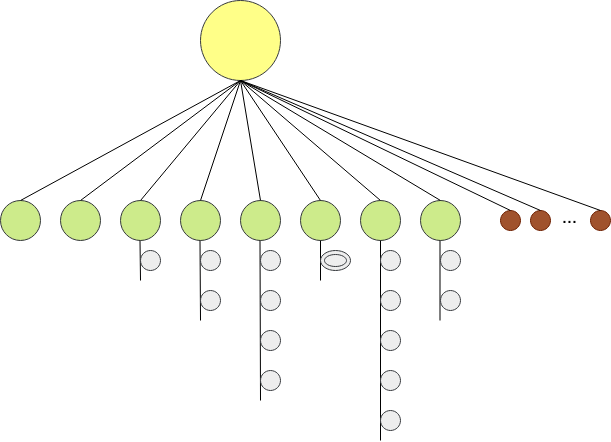
\includegraphics[scale=0.6]{tree_struct.png}
\caption{Visão geral da estrutura principal Tree.}
\label{img:tree_struct}
\end{figure}


\subsection{Tree}
\label{sec:tree}

A classe Tree será usada para representar uma Árvore. Uma instância de Árvore tem uma \textbf{Figure} principal e um \textbf{vector} com os \textit{filhos} que tem.

\begin{figure}[H]
\centering
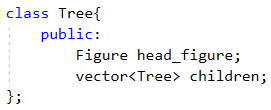
\includegraphics[scale=0.8]{tree.png}
\caption{Estrutura que define instâncias de uma Árvore}
\label{img:Tree}
\end{figure}


\subsection{Figure}
\label{sec:figure}

A classe Figure é composta por um inteiro com o número de triângulos que constitui essa figura, um vector com os pontos todos da figura. Possui também as 3 transformações geométricas que são feitas sobre a mesma - Translation, Rotation, Scale. Contém ainda uma Color, para definir a cor da figura.

\begin{figure}[H]
\centering
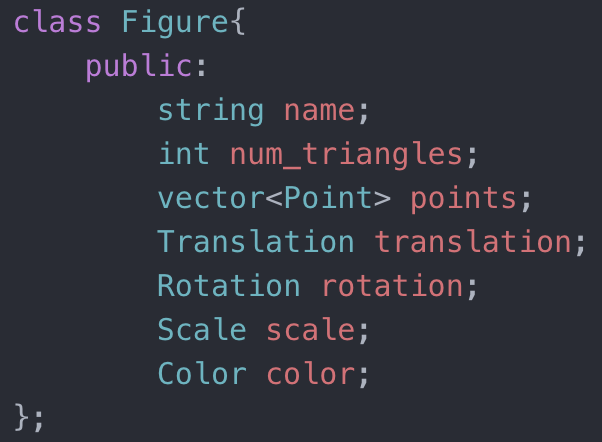
\includegraphics[scale=0.8]{figure.png}
\caption{Estrutura que define instâncias de uma Figura}
\label{img:Figure}
\end{figure}


\subsection{Color}
\label{sec:color}

A classe Color é composta por 3 floats - r,g e b. Estes floats juntos definem a cor para usar numa figura.

\begin{figure}[H]
\centering
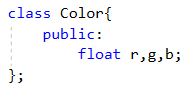
\includegraphics[scale=0.8]{color.png}
\caption{Estrutura que define instâncias de Cor.}
\label{img:Color}
\end{figure}


\subsection{Scale}
\label{sec:scale}

A classe Scale contém 3 floats - x,y e z, que são os parâmetros de redimensionamento da figura que queremos. Contém ainda um bool para verificar se a transformação existe.

\begin{figure}[H]
\centering
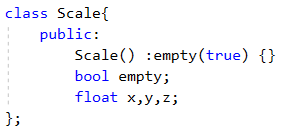
\includegraphics[scale=0.8]{scale.png}
\caption{Estrutura que define instâncias de Scale}
\label{img:Scale}
\end{figure}

\newpage

\subsection{Rotation}
\label{sec:rotation}

A classe Rotation é composta por 4 floats - as coordenadas dos eixos e o ângulo que queremos rodar a figura. Tem também um bool empty que apenas permite a leitura caso o seu valor seja true.

\begin{figure}[H]
\centering
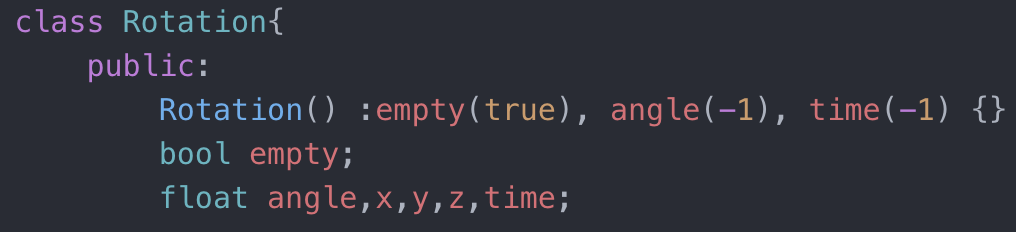
\includegraphics[scale=0.8]{rotation.png}
\caption{Estrutura que define instâncias de Rotation}
\label{img:Rotation}
\end{figure}


\subsection{Translation}
\label{sec:translation}

A classe Translation é também composta pelas 3 coordenadas dos eixos e pela verificação de que a figura existe mesmo e queremos lê-la.

\begin{figure}[H]
\centering
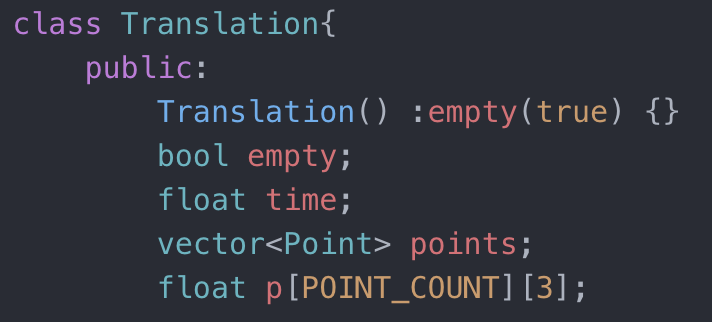
\includegraphics[scale=0.8]{translation.png}
\caption{Estrutura que define instâncias de Translation}
\label{img:Tree}
\end{figure}


\subsection{Point}
\label{sec:point}

A classe Point, como o nome indica, é um ponto no sistema, ou seja, é composta por 3 floats - x, y e z.

\begin{figure}[H]
\centering
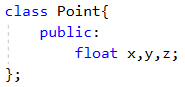
\includegraphics[scale=0.8]{point.png}
\caption{Estrutura que define instâncias de Point}
\label{img:Point}
\end{figure}


\newpage

\section{\textit{Render Scene}}
Para o rendering do projeto, utilizamos uma pesquisa em profundidade na árvore representando  todas as figuras e as suas translações, rotações e escalas.

Assim, a função renderScene(), chama duas funções. A função drawAxis() que representa os 3 eixos de coordenadas na cena e a função drawTree que desenha o conteúdo da árvore.

Esta função drawTree recebe como pârametro uma árvore (Tree) e o seu algoritmo pode ser explicado assim:


\ttfamily
\begin{enumerate}
 \item Efetua o push inicial  $\Rightarrow$ \textit{glPushMatrix()};
 \item Verifica se a figura atual tem alguma translação;
    \begin{enumerate}
      \item Caso tenha, efetua a translação com a \textit{glTranslatef()};
    \end{enumerate}
  \item Verifica se a figura atual tem alguma rotação;
    \begin{enumerate}
      \item Caso tenha, efetua a translação com a \textit{glRotatef()};
    \end{enumerate}
 \item Verifica se a figura atual tem alguma escala;
    \begin{enumerate}
      \item Caso tenha, efetua a translação com a \textit{glScalef()};
    \end{enumerate}
 \item Após as transformações geométricas serem feitas, através da \textit{drawFigure(}), é desenhada a figura do nodo atual.
 \item Para o vector de filhos é invocada recursivamente a função \emph{drawTree(filho)}. Desta forma asseguramos a hereditariedade das figuras.
 \item Finalizando, é efetuado o \textit{glPopMatrix()};
\end{enumerate}

\rmfamily

  \vspace{0.3cm}

 A função \textit{drawFigure()}, que tem como pârametro uma \textbf{Figure}, é responsável por desenhar uma figura e o seu algoritmo pode ser explicado assim:

\ttfamily

  \vspace{0.3cm}

\begin{enumerate}
 \item Colocar num \textit{vector<Point>} todos os pontos que compõem a figura;
 \item Colocar numa estrutura Color, a cor da figura;
 \item Iniciar o desenho com \textit{glBegin(GL\_TRIANGLES)} e com \textit{glColor3f(com os parâmetros que colocamos na estrutura Color0});
 \item Iterando sobre o vector dos pontos:
	\begin{enumerate}
	\item Colocar numa estrutura Point, o ponto actual da iteração (current\_point);
	\item Através da \textit{glVertex3f(current\_point.x,current\_point.y,current\_point.z)} desenhar o ponto atual;
	\end{enumerate}
\item Terminada a iteração, termina o desenho da figura com \textit{glEnd()};
\end{enumerate}

\rmfamily

\newpage

\section{\textit{Generator}}

Nesta segunda fase do projeto usamos o programa criado na primeira fase (\textbf{Generator}) para criar todas as figuras com o intuito de alimentar os ficheiros \emph{XML} e consequentemente o programa \textbf{Engine}.

\subsection{Cintura de Asteróides}

Para além da sua funcionalidade inicial, achamos que seria benéfico para o nosso modelo estático do sistema solar ter uma cintura de asteróides. Tal tarefa era bastante difícil de realizar, asteróide a asteróide, pelo que decidimos adicionar uma nova funcionalidade ao \textbf{Generator}. Esta funcionalidade passa por gerar um ficheiro \emph{XML} com o formato definido na secção \textbf{\ref{sec:ficheiro}} que contém todos os asteróides pertencentes à cintura de asteróides entre Marte e Júpiter.

Depois de ter o ficheiro com a cintura de asteróides gerada, temos que copiar o conteúdo deste ficheiro e colocá-lo corretamente no ficheiro \emph{scene.xml} que é onde reside todo o modelo do sistema solar.

Um exemplo de como invocar esta função é:

 \vspace{0.5cm}

$\Rightarrow$ ./Generator asteroid\_belt 1000 150 160 asteroids.xml

 \vspace{0.5cm}

 Neste caso vamos gerar \emph{XML} que será escrito no ficheiro \textbf{\emph{asteroids.xml}}, que irá conter \textbf{1000} asteróides a uma distância do sol compreendida entre \textbf{150} e \textbf{160}.

O algoritmo utilizado é descrito a seguir.

\subsubsection{Algoritmo}
A função \textit{generateAsteroids} recebe como parâmetro três inteiros que representam respetivamente, o número de asteróides a criar, o raio mínimo e o raio máximo a que estão do sol. Por último recebe o nome do ficheiro onde irá guardar o \emph{XML} criado.

De seguida apresentamos uma imagem duma cintura de asteróides gerada pela nossa aplicação e a sua explicação através do algoritmo criado pelo grupo.

 \ttfamily
\begin{enumerate}
  \item Inicializa-se um gerador de números pseudo-aleatórios, usando 1 como \emph{seed} $\Rightarrow$ srand(1).
  \item Iterar sobre o número de asteróides:
  \begin{enumerate}
    \item Enquanto não for gerado um ponto válido:
    \begin{enumerate}
    	\item Calcula-se um número aleatório para X, baseando-se na fórmula:

	 \vspace{0.5cm}

	 \hspace{0.0cm} X $\Rightarrow$ rand() \% (2 $\times$ raio máximo) - raio máximo

	 \vspace{0.5cm}

	 \item Calcula-se um número aleatório para Z, baseando-se na fórmula:

	 \vspace{0.5cm}

	 \hspace{0.0cm} Z $\Rightarrow$ rand() \% (2 $\times$ raio máximo) - raio máximo

	 \vspace{0.5cm}

	 \item Calcula-se a distância ao centro, calculando a hipotenusa:

	 \vspace{0.5cm}

	 \hspace{0.0cm} Hipotenusa $\Rightarrow$ $\sqrt{X^2 + Z^2}$

	 \vspace{0.5cm}

	 \item Testa-se se a hipotenusa está compreendida entre o raio mínimo e o raio máximo.
	 \begin{enumerate}
	 \item Se sim, escreve em ficheiro e passa à próxima iteração para um novo asteróide.
	 \item Se não, entra no ciclo até tentar ter um ponto válido.
	 \end{enumerate}

    \end{enumerate}

    \end{enumerate}

    \item Fim
    \end{enumerate}
    \rmfamily


\begin{figure}[H]
\centering
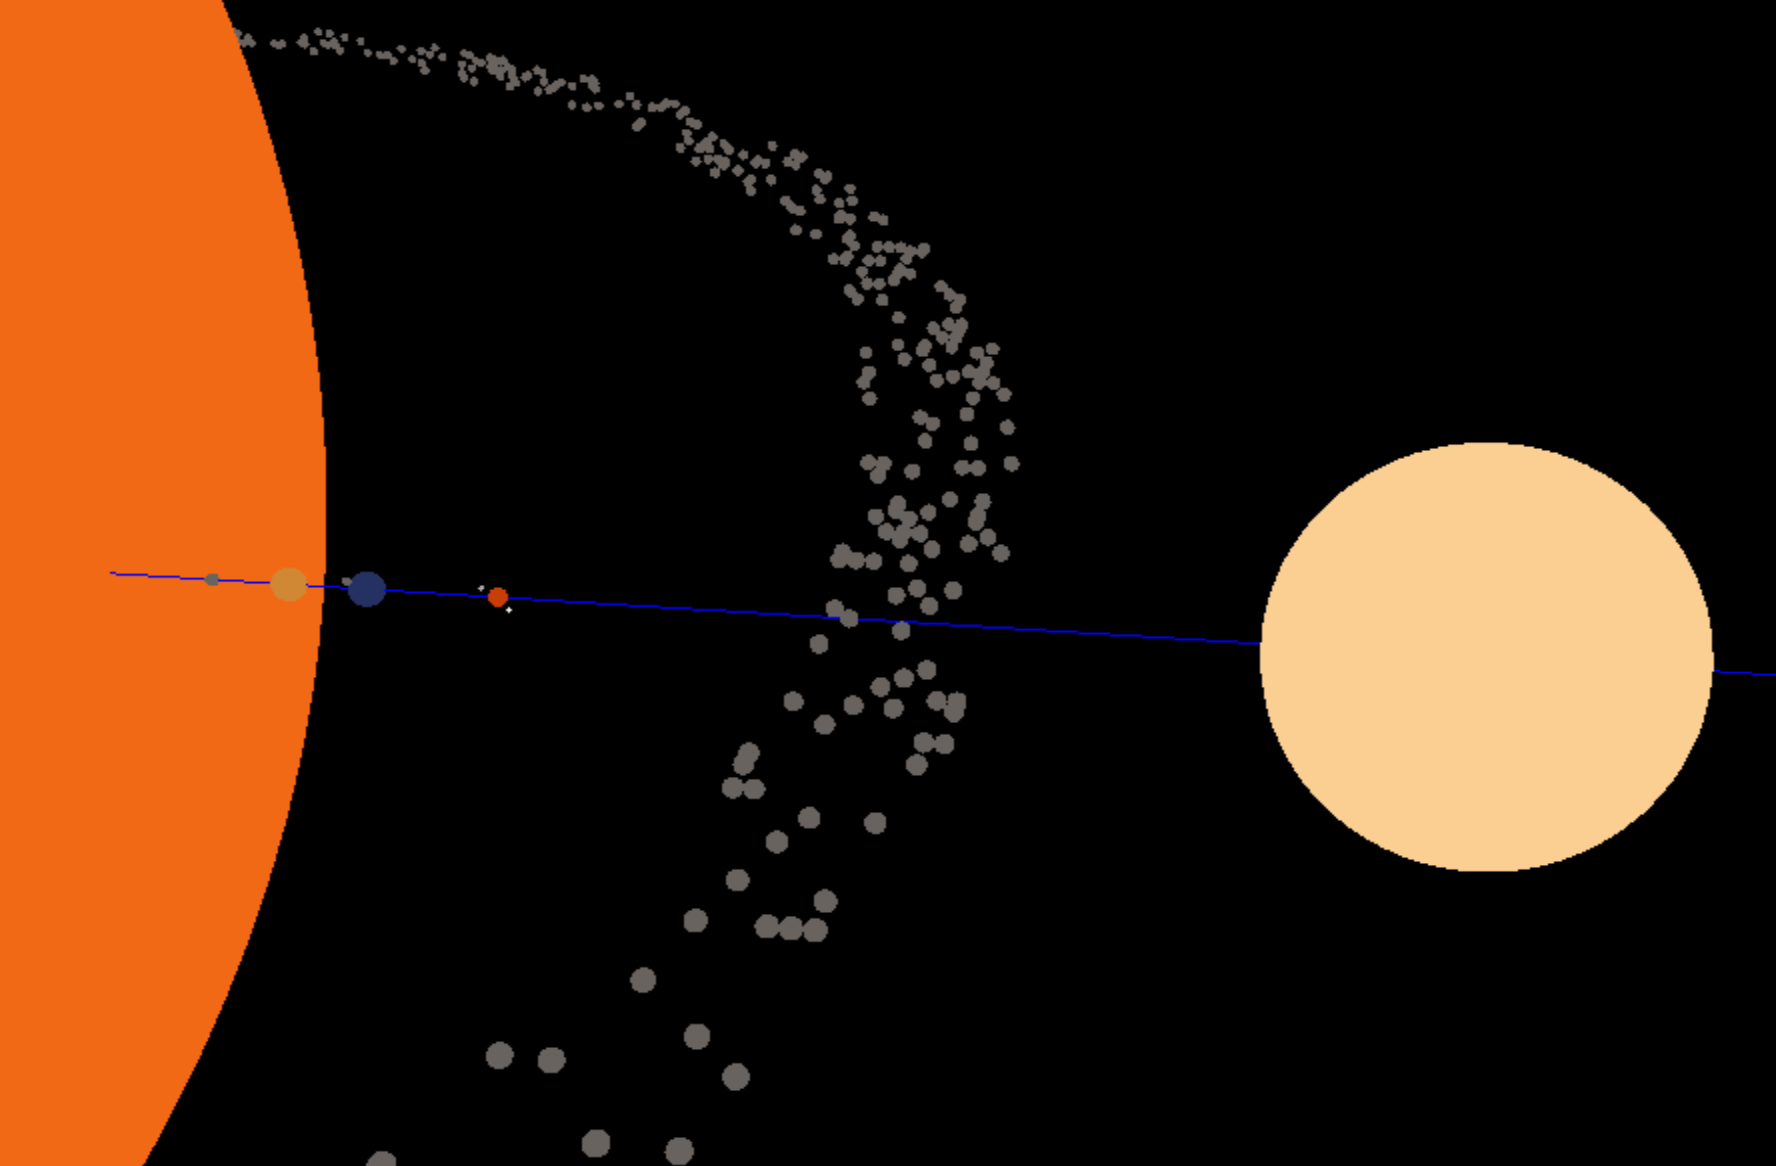
\includegraphics[scale=0.45]{cintura.png}
\caption{Imagem exemplificativa duma cintura de asteróides}
\label{img:cintura}
\end{figure}



\subsection{Torus}

Como Saturno na sua verdadeira natureza possui um anel, achamos por bem que o nosso modelo do sistema solar deveria conter algo que o representasse, uma vez que esta é uma característica bem conhecida deste planeta. Para tal achamos que uma \emph{Torus} representaria bem o que pretendíamos.

Desta forma, criamos uma nova funcionalidade para o \textbf{Generator} que possibilita a criação de todos os pontos necessários para a criação duma \emph{Torus}.

Um exemplo de como invocar esta função é:

 \vspace{0.5cm}

$\Rightarrow$ ./Generator torus 0.3 1.5 20 30 torus.3d

 \vspace{0.5cm}

 Neste caso iremos os pontos para a figura que serão guardados no ficheiro \textbf{torus.3d}, o raio de cada anel será de \textbf{0.3}, a distância (raio) do centro da figura até à figura será \textbf{1.5}, o número de lados de cada anel será \textbf{20} e finalmente o número de anéis que compõe a figura será \textbf{30}.

 \subsubsection{Algoritmo}

 \ttfamily
\begin{enumerate}
  \item Definir o avanço de $\phi$ em cada iteração: $$delta\phi = \frac{2\pi}{numero\ rings} $$
  \item Definir o avanço de $\theta$ em cada iteração: $$delta\theta = \frac{2\pi}{numero\ sides} $$
  \item Iterar sobre o número de rings:
  \begin{enumerate}
    \item Calcular o ângulo phi para o ring atual $\Rightarrow$ \underline{$delta\phi \times ring\ atual$}
    \item Calcular o ângulo nextPhi para o ring seguinte $\Rightarrow$ \underline{$delta\phi \times ring\ seguinte$}
    \item Calcular o cosPhi $\Rightarrow$ \underline{$cos(phi)$}
    \item Calcular o sinPhi $\Rightarrow$ \underline{$sin(phi)$}
    \item Calcular o cosNextPhi $\Rightarrow$ \underline{$cos(nextPhi)$}
    \item Calcular o sinNextPhi $\Rightarrow$ \underline{$sin(nextPhi)$}

    \vspace{0.2cm}

    \item Iterar sobre o número de sides:
    \begin{enumerate}
      \item Calcular o ângulo theta para o side atual $\Rightarrow$ \underline{$delta\theta \times side\ atual$}
      \item Calcular o ângulo nextTheta para o side seguinte $\Rightarrow$ \underline{$delta\theta \times side\ seguinte$}
      \item Calcular o cosTheta $\Rightarrow$ \underline{$cos(theta)$}
      \item Calcular o sinTheta $\Rightarrow$ \underline{$sin(theta)$}
      \item Calcular o cosNextTheta $\Rightarrow$ \underline{$cos(nextTheta)$}
      \item Calcular o sinNextTheta $\Rightarrow$ \underline{$sin(nextTheta)$}
      \item Calcular o distancia ao ponto:

       \vspace{0.2cm}

       $\Rightarrow$ \underline{$ dXZ = outerRadius + innerRadius \times cosTheta$}

       \vspace{0.5cm}

      \item Calcular o distancia ao ponto do side seguinte:

      \vspace{0.2cm}

      $\Rightarrow$ \underline{$ nextDXZ = outerRadius + innerRadius \times cosNextTheta$}

      \vspace{0.5cm}

      \item Construir os dois triângulos do side atual:

      \vspace{0.3cm}

      \underline{Primeiro triângulo:}

      \vspace{0.3cm}

          \hspace{-2.0cm} P1 $\Rightarrow$ ($nextDXZ \times cosPhi , innerRadius \times sinNextTheta , nextDXZ \times sinPhi$)

      \vspace{0.2cm}

          \hspace{-1.8cm} P2 $\Rightarrow$ ($dXZ \times cosNextPhi , innerRadius \times sinTheta , dXZ \times sinNextPhi$)

      \vspace{0.2cm}

          \hspace{-1.5cm} P3 $\Rightarrow$ ($dXZ \times cosPhi , innerRadius \times sinTheta , dXZ \times sinPhi$))

      \vspace{0.3cm}

      \underline{Segundo triângulo:}

      \vspace{0.3cm}

          \hspace{-3.0cm} P1 $\Rightarrow$ ($nextDXZ \times cosNextPhi, innerRadius \times sinNextTheta, nextDXZ \times sinNextPhi$)

      \vspace{0.2cm}

          \hspace{-2.3cm} P2 $\Rightarrow$ ($dXZ \times cosNextPhi, innerRadius \times sinTheta, dXZ \times sinNextPhi$)

      \vspace{0.2cm}

          \hspace{-2.5cm} P3 $\Rightarrow$ ($nextDXZ \times cosPhi, innerRadius \times sinNextTheta, nextDXZ \times sinPhi$)

      \vspace{0.2cm}

    \end{enumerate}

    \end{enumerate}

    \item Fim
    \end{enumerate}
    \rmfamily

\begin{figure}[H]
\centering
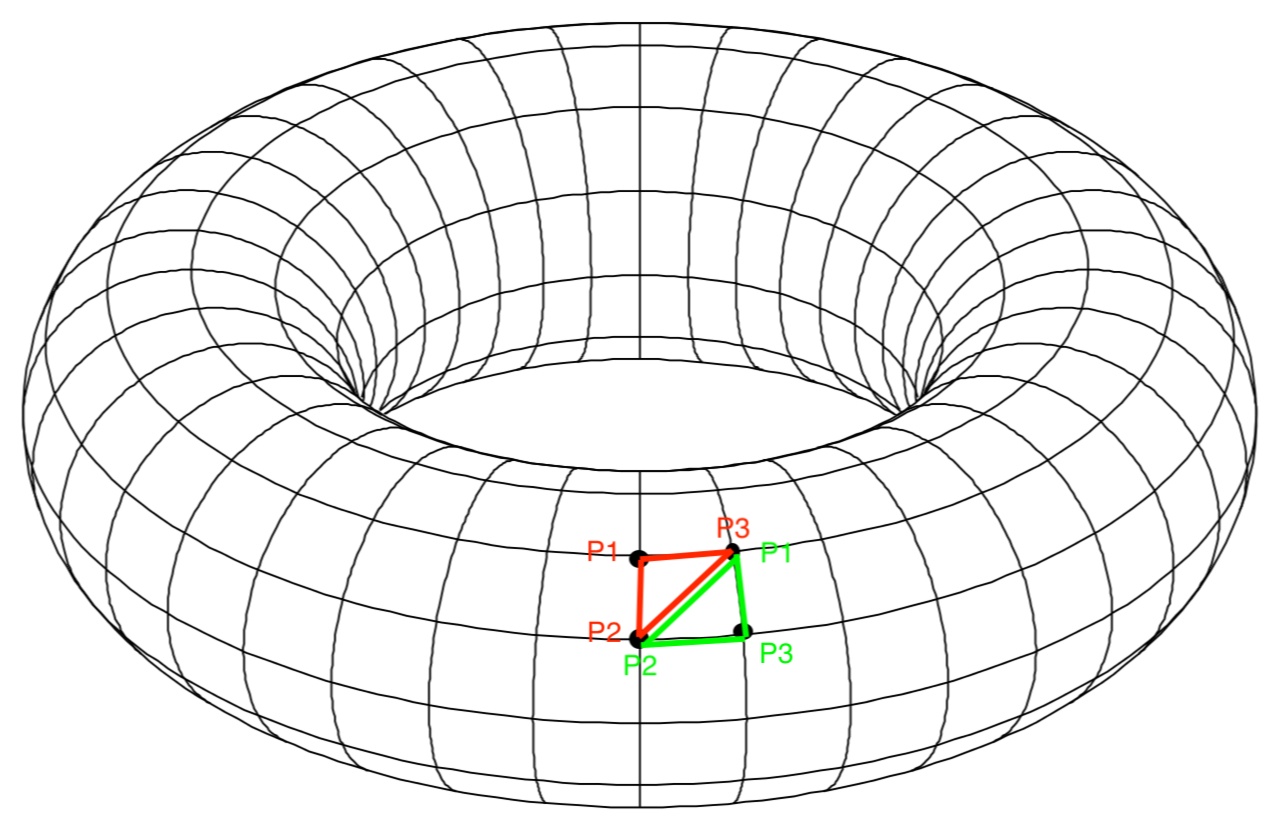
\includegraphics[scale=0.3]{torus_triangulos.png}
\caption{Triângulos gerados por iteração.}
\label{img:torus_triangulos}
\end{figure}

Na figura \ref{img:torus_triangulos} o triângulo que se encontra a \textbf{verde} é o \textbf{primeiro} a ser gerado, baseando-nos no algoritmo apresentado acima. Consequentemente o triângulo que se encontra a \textbf{vermelho} é o \textbf{segundo} a ser gerado.



\newpage


\section{Upgrades da Fase Anterior}

Em relação à fase anterior houve alguns pontos que foram sujeitos a mudanças e otimizações pelo que estas serão relatadas nesta secção.

Uma das partes que foi sujeita a otimização foi o cálculo das coordenadas da câmera que na fase anterior continha demasiado código e algumas variáveis que não tinham nexo em ser usadas.
Desta forma decidimos que esta parte deveria ser reescrita utilizando uma abordagem mais objetiva. O resultado é descrito na seguinte figura.

\begin{figure}[H]
\centering
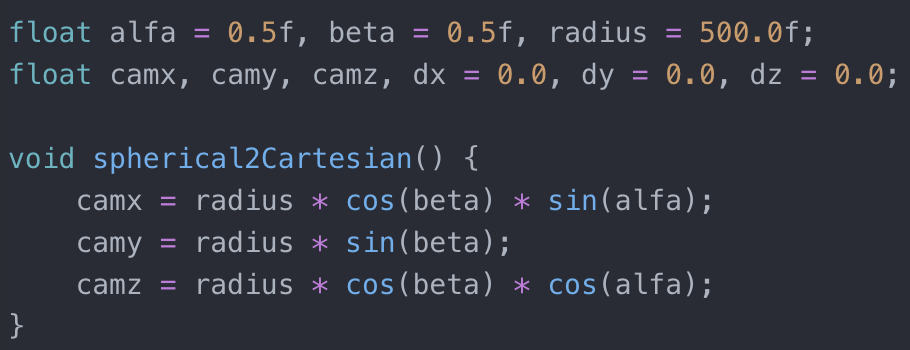
\includegraphics[scale=0.7]{camara.png}
\caption{Código referente às coordenadas da câmara.}
\label{img:camara}
\end{figure}

Não só a função que calcula as coordenadas para câmara mas também a própria função da câmara foi melhorada. Passou a poder mover-se consoante o ponto para o qual está a olhar. Desta forma possibilitou-nos a facilidade de podermos deslocarmo-nos para qualquer sítio que nos convenha. Tal alteração é descrita na seguinte figura.

\begin{figure}[H]
\centering
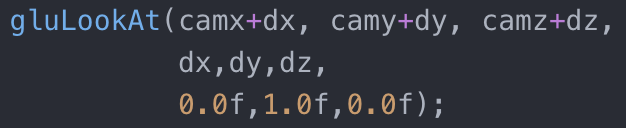
\includegraphics[scale=0.7]{mat_camara.png}
\caption{Função que contém a matriz da câmara.}
\label{img:mat_camara}
\end{figure}

Outra das partes que sofreu algumas alterações foi a organização do código na pasta \textbf{Generator} que estava definido em ficheiros \emph{.h} (plane, box, sphere e cone). Não devendo então código ser escrito em ficheiros deste género, excetuando apenas as definições e documentação, criamos um ficheiro \emph{.h} que alberga todas as definições e documentação necessária e criamos ficheiros \emph{.cpp} para cada figura. Desta forma todo o código ficou perfeitamente organizado.


\newpage

\section{\textit{Scenes}}

Nesta fase do projeto é requerido um modelo estático do sistema solar, com o sol, os planetas e os satélites naturais do mesmo.

  \vspace{0.5cm}

O grupo decidiu proceder à criação de duas cenas do sistema solar:

\begin{enumerate}
\item Modelo baseado nas diferenças reais entre os raios dos corpos presentes.
\item Modelo mais elucidativo e perceptível, que despreza parcialmente as diferenças reais entre os corpos presentes.
\end{enumerate}

  \vspace{0.5cm}

Na execução do programa \textit{Engine} são disponibilizadas essas duas opções, e o utilizador deve escolher a que pretende visualizar. Deve, portanto, inserir o número do modelo que pretende. De seguida, na figura \ref{img:interface}, é exemplificado um possível procedimento.

\begin{figure}[H]
\centering
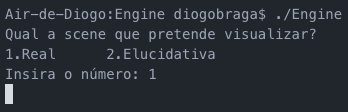
\includegraphics[scale=0.7]{interface.png}
\caption{Exemplo de um possível procedimento na interface.}
\label{img:interface}
\end{figure}


\newpage

\subsection{Primeiro Modelo}

\begin{figure}[H]
\centering
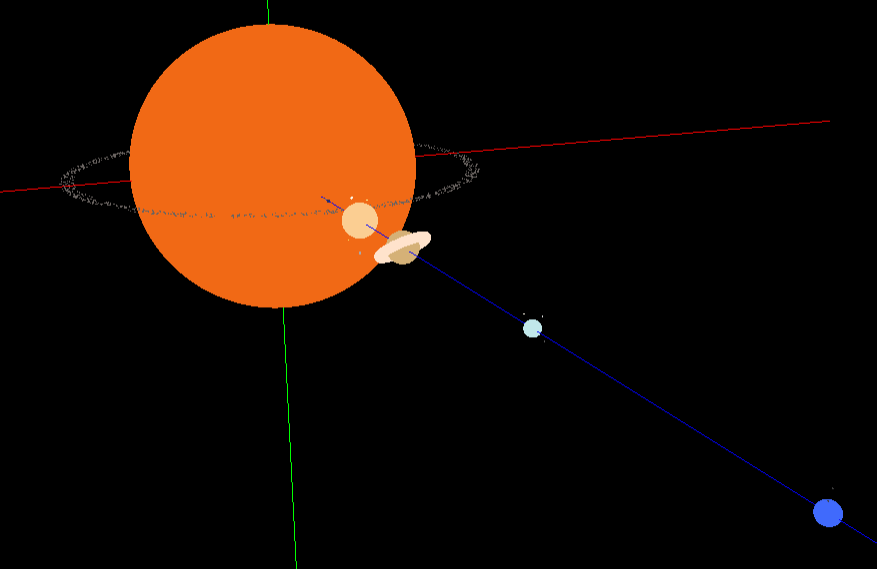
\includegraphics[scale=0.4]{modelo1_1.png}
\caption{Imagem total do primeiro modelo.}
\label{img:modelo1_1}
\end{figure}

\begin{figure}[H]
\centering
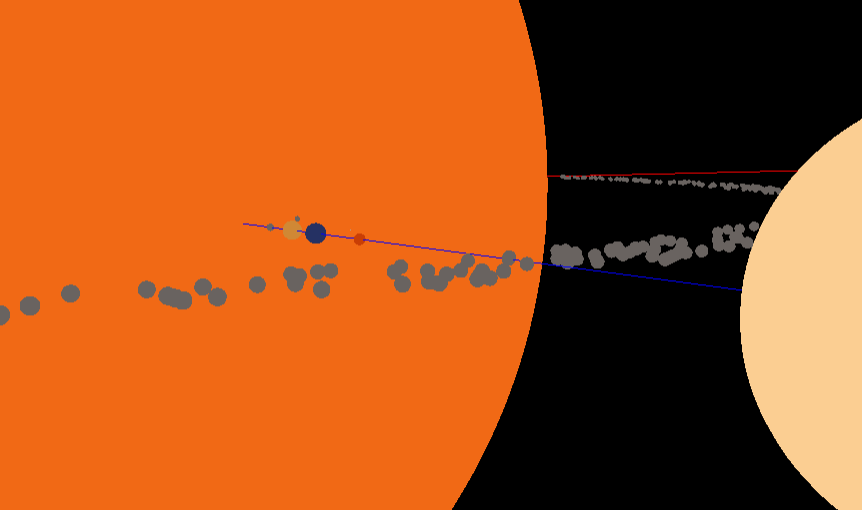
\includegraphics[scale=0.4]{modelo1_2.png}
\caption{Imagem parcial do primeiro modelo.}
\label{img:modelo1_2}
\end{figure}


\newpage

\subsection{Segundo Modelo}

\begin{figure}[H]
\centering
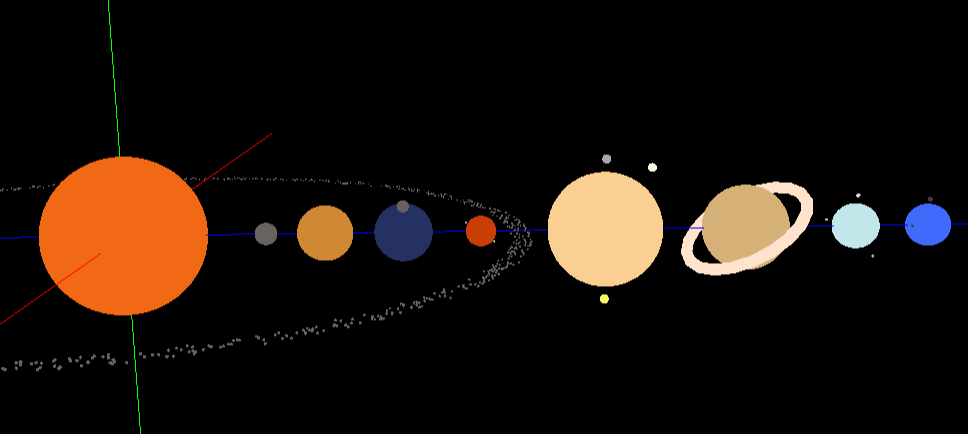
\includegraphics[scale=0.4]{modelo2_1.png}
\caption{Imagem frontal do segundo modelo.}
\label{img:modelo2_1}
\end{figure}

\begin{figure}[H]
\centering
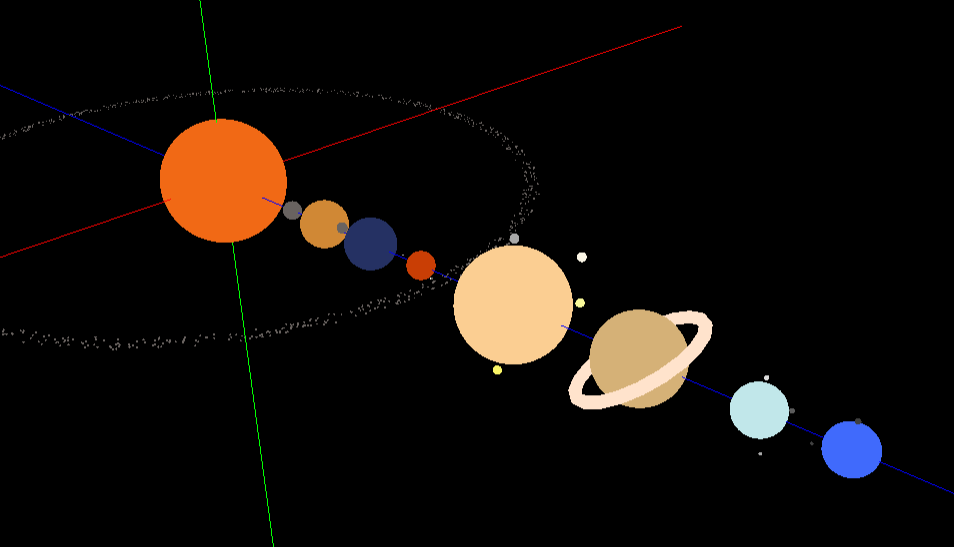
\includegraphics[scale=0.4]{modelo2_2.png}
\caption{Imagem lateral do segundo modelo.}
\label{img:modelo2_2}
\end{figure}


\newpage

\section{Conclusão}
\label{sec:conclusao}

Após a conclusão desta fase do projeto, todos os membros do grupo se sentem mais à vontade com transformações geométricas e, consequentemente, com todos os conceitos apreendidos nas aulas que tiveram de ser colocados em prática nesta fase.

A implementação de estruturas mais elaboradas para aproveitar o conceito de hereditariedade de figuras foi algo enriquecedor em termos de programação e melhorou consideravelmente a performance do projeto.

Relativamente ao nível de execução desta fase o grupo, no geral, não sentiu grandes dificuldades.

Em jeito de conclusão e revisão final a esta fase, o grupo espera continuar num bom caminho para a realização de todas as fases deste projeto, que, para já, tem sido um projeto prazeroso.

\section{Bibliografia}
\label{sec:bibliografia}

\begin{itemize}

  \item \textbf{Planetary Pixels Emporium :}
  \begin{itemize}
    \item https://www.suapesquisa.com/astronomia/distancia\_sol\_planetas.htm
  \end{itemize}
  \item \textbf{123RF : (Diagrama do Sistema Solar)}
  \begin{itemize}
    \item https://www.123rf.com/photo\_43149668\_stock-vector-diagram-of-solar-system.html
  \end{itemize}
  \item \textbf{Site Astronomia}
  \begin{itemize}
    \item http://www.siteastronomia.com/distancia-e-tamanho-dos-planetas-do-sistema-solar
  \end{itemize}

\end{itemize}

\end{document}
